Dans cette partie nous allons résoudre (1) à l'aide de discrétisation et de différences finies. Puis nous résoudrons celle-ci à l'aide des transformées de Fourier. \\
\subsubsection{Qu'est qu'une image}
Avant de résoudre numériquement le problème, nous rappelons ce qu'est un image et comment nous la  parcourrons dans la suite.\\
Une image peut être représentée comme une succession de pixels. En traitement d'image, ce sont d'ailleurs sur ces pixels que le traitement est effectué. Leur modification entraîne la modification de l'image globale.Il est alors possible de découper l'image, en prenant comme échelle le pixel. L'image peut donc être vue comme une grille, dans laquelle chaque carré représente un pixel. Les pixels seront numérotés suivant la règle suivante : \\

Le premier pixel est situé en haut en gauche, puis il suffit de parcourir la grille, de gauche à droite et de haut en bas, comme ci-dessous :  
\begin{figure}[!htb]
   \begin{minipage}{0.5\textwidth}
     \centering
     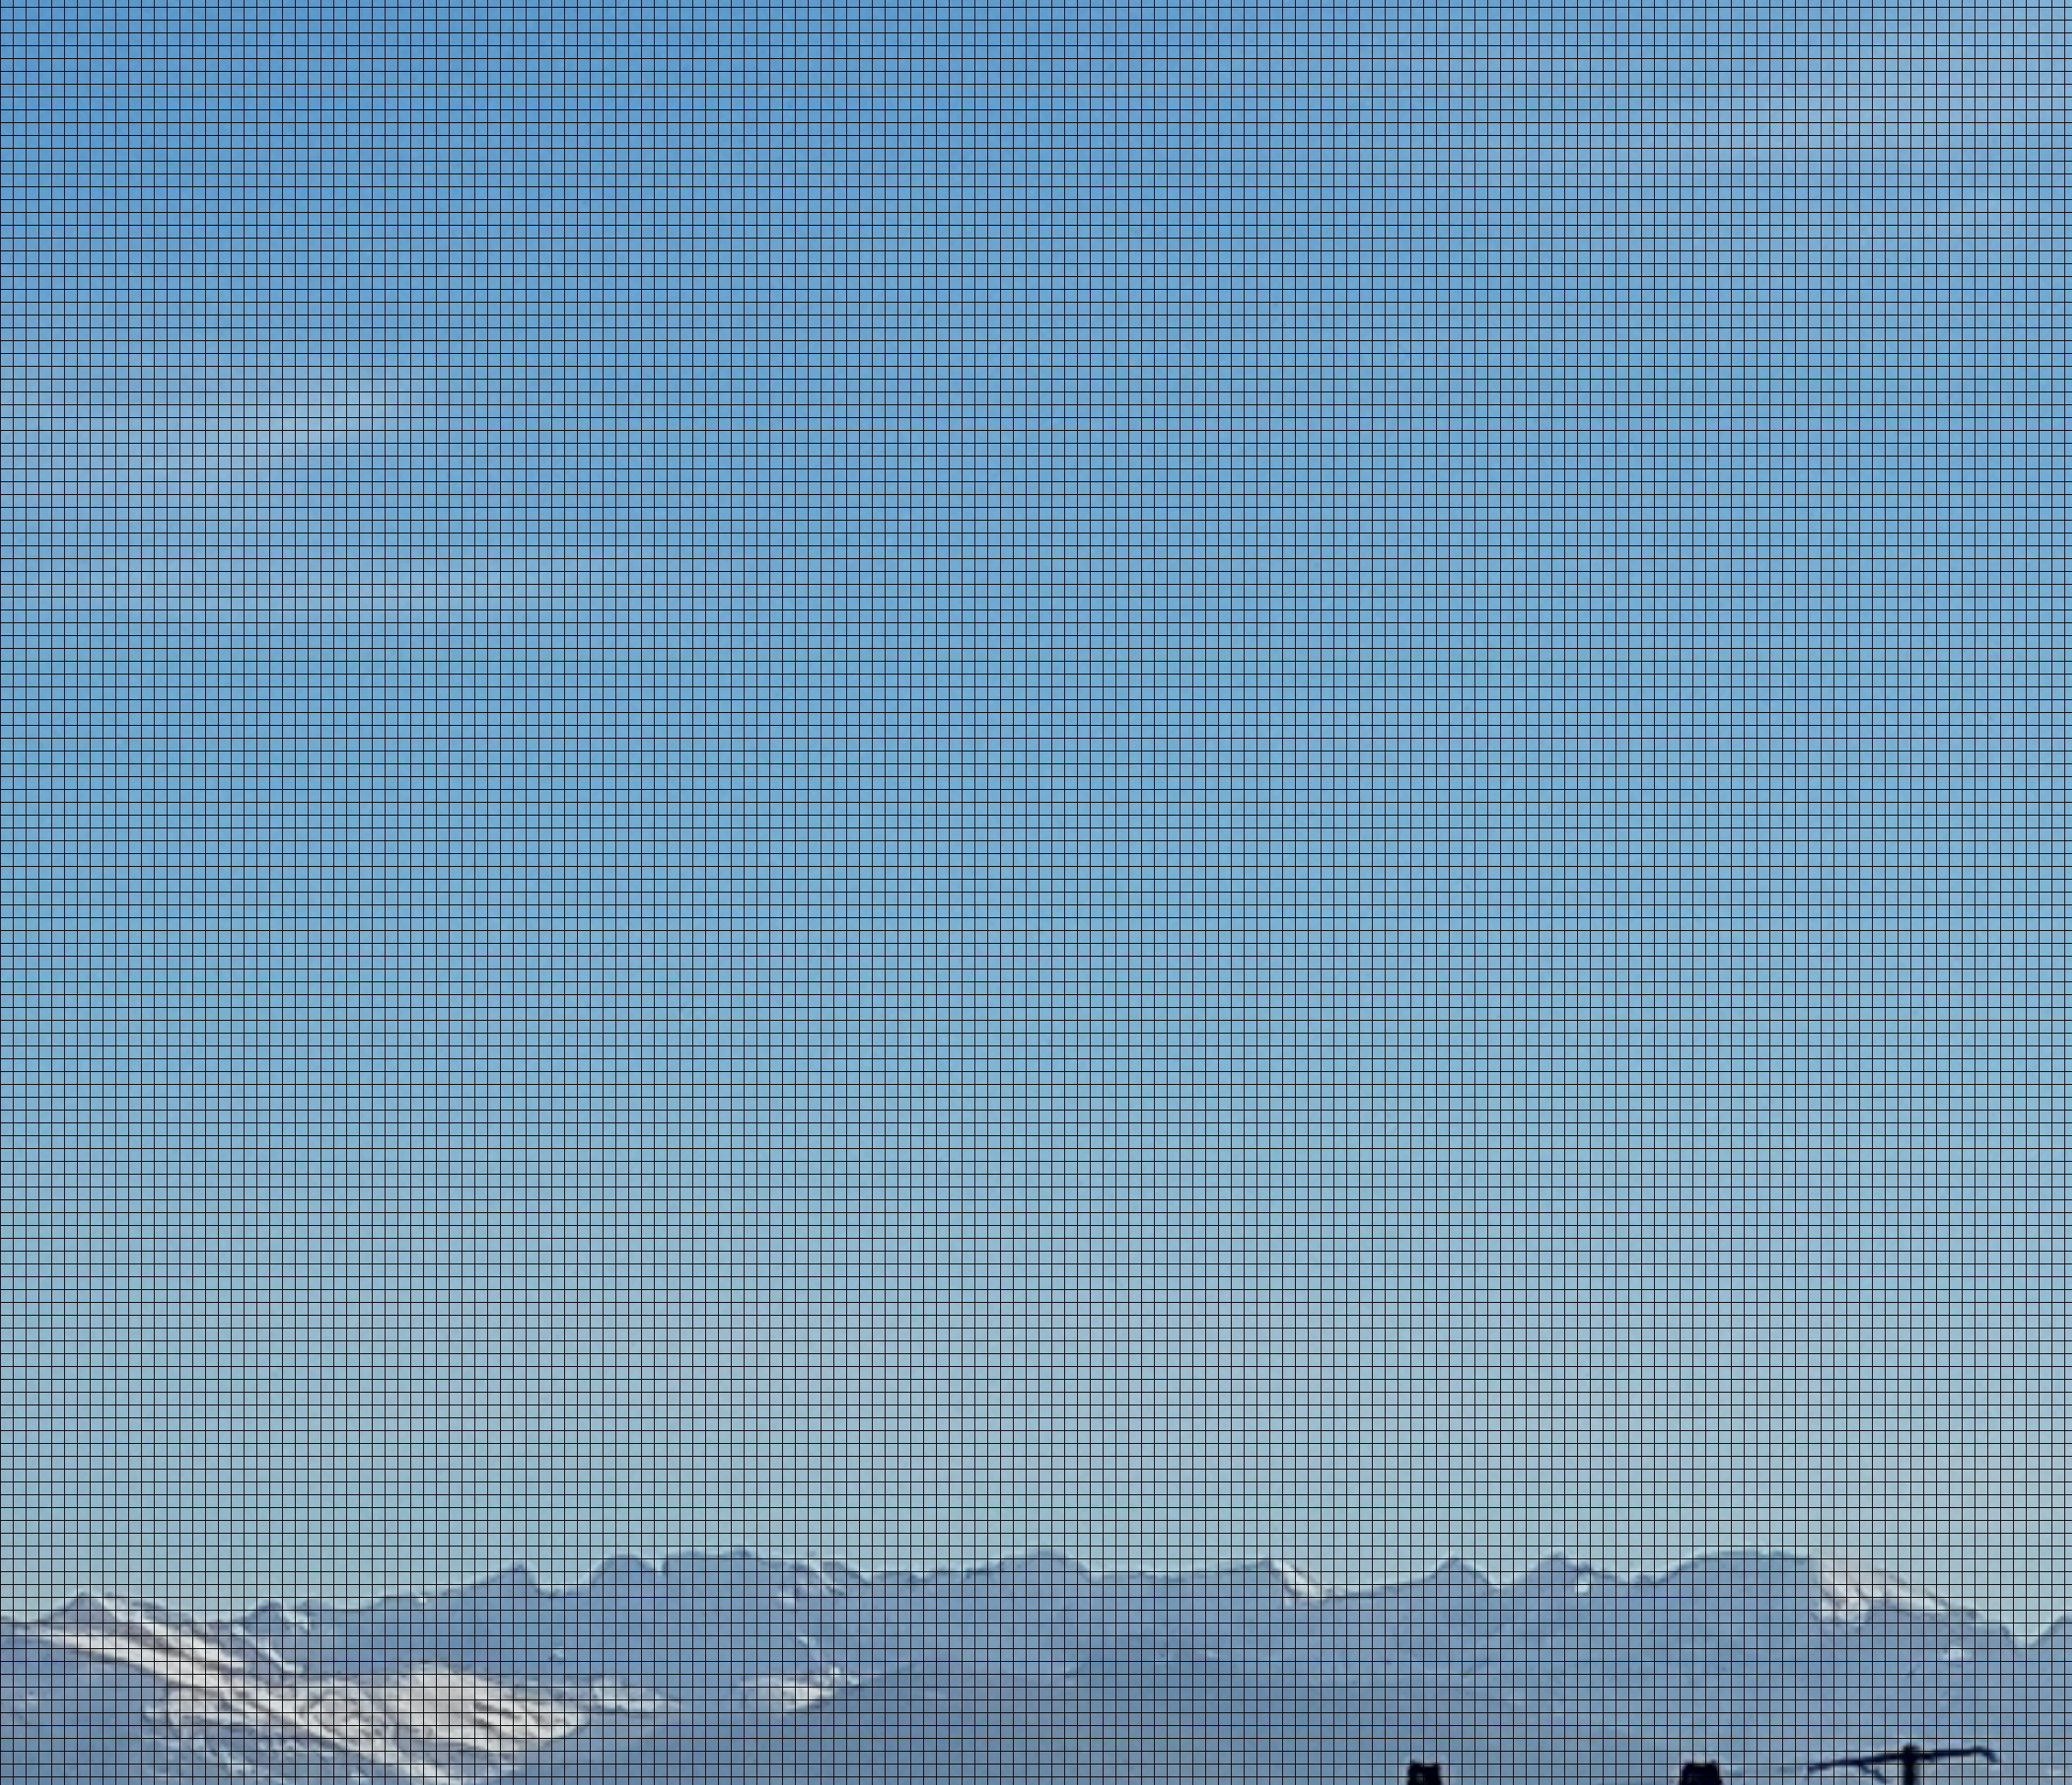
\includegraphics[width = 120pt]{Images/Montagne_grille.jpg}
        \caption{Maillage d'une image}
      \end{minipage}\hfill
   \begin{minipage}{0.5\textwidth}
     \centering
     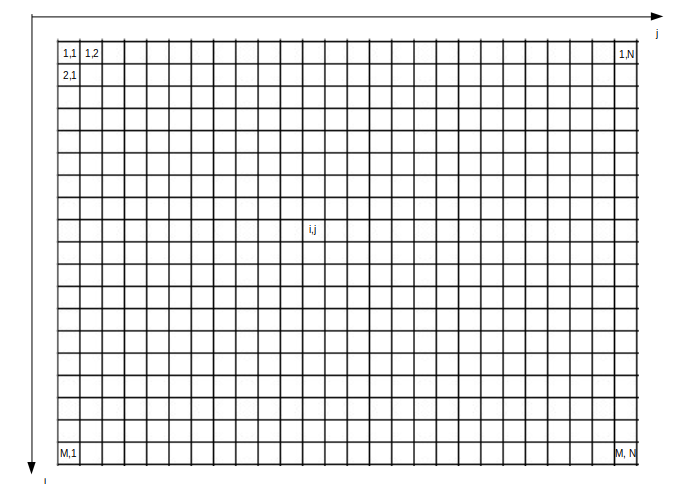
\includegraphics[width = 120pt]{Images/grille.png}
	\caption{Parcours d'une grille}
      \end{minipage}\hfill
\end{figure}

Les pas d'espaces sont donc égaux et valent 1. Dans la suite nous considérerons que l'image à modifier est de taille $M \times N$.

